\begin{figure}[h]
 \center
 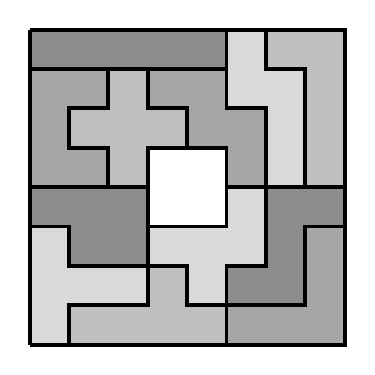
\begin{tikzpicture}[scale = 0.5]
  \draw[help lines] (0, 0) grid (8, 8);
  \draw[line width=0.5mm, fill=black!15] (0, 0) -- (1, 0) -- (1, 1) -- (3, 1) -- (3, 2) -- (1, 2) -- (1, 3) -- (0, 3) -- (0, 0);
  \draw[line width=0.5mm, fill=black!25] (1, 0) -- (5, 0) -- (5, 1) -- (4, 1) -- (4, 2) -- (3, 2) -- (3, 1) -- (1, 1) -- (1, 0);
  \draw[line width=0.5mm, fill=black!35] (5, 0) -- (8, 0) -- (8, 3) -- (7, 3) -- (7, 1) -- (5, 1) -- (5, 0);
  \draw[line width=0.5mm, fill=black!45] (0, 3) -- (1, 3) -- (1, 2) -- (3, 2) -- (3, 4) -- (0, 4) -- (0, 3);
  \draw[line width=0.5mm, fill=black!15] (3, 2) -- (4, 2) -- (4, 1) -- (5, 1) -- (5, 2) -- (6, 2) -- (6, 4) -- (5, 4) -- (5, 3) -- (3, 3) -- (3, 2);
  \draw[line width=0.5mm, fill=black!45] (5, 1) -- (7, 1) -- (7, 3) -- (8, 3) -- (8, 4) -- (6, 4) -- (6, 2) -- (5, 2) -- (5, 1);
  \draw[line width=0.5mm, fill=black!35] (0, 4) -- (2, 4) -- (2, 5) -- (1, 5) -- (1, 6) -- (2, 6) -- (2, 7) -- (0, 7) -- (0, 4);
  \draw[line width=0.5mm, fill=black!25] (2, 4) -- (3, 4) -- (3, 5) -- (4, 5) -- (4, 6) -- (3, 6) -- (3, 7) -- (2, 7) -- (2, 6) -- (1, 6) -- (1, 5) -- (2, 5) -- (2, 4);
  \draw[line width=0.5mm, fill=black!35] (3, 6) -- (4, 6) -- (4, 5) -- (5, 5) -- (5, 4) -- (6, 4) -- (6, 6) -- (5, 6) -- (5, 7) -- (3, 7) -- (3, 6);
  \draw[line width=0.5mm, fill=black!15] (5, 6) -- (6, 6) -- (6, 4) -- (7, 4) -- (7, 7) -- (6, 7) -- (6, 8) -- (5, 8) -- (5, 6);
  \draw[line width=0.5mm, fill=black!25] (7, 4) -- (8, 4) -- (8, 8) -- (6, 8) -- (6, 7) -- (7, 7) -- (7, 4);
  \draw[line width=0.5mm, fill=black!45] (0, 8) -- (5, 8) -- (5, 7) -- (0, 7) -- (0, 8);
  \draw[line width=0.5mm, fill=gray!0] (3, 3) -- (3, 5) -- (5, 5) -- (5, 3) -- (3, 3);
 \end{tikzpicture}

 \caption{一个方块覆盖问题的实例}
 \label{fig:tetris}
\end{figure}
